\documentclass[12pt]{article}

% UTF-8 encoding and fonts
\usepackage[utf8]{inputenc}
\usepackage[T1]{fontenc}
\usepackage{lmodern}  % Latin Modern font - fixes < > rendering issues

% Page setup
\usepackage[margin=1in]{geometry}
\usepackage{setspace}
\onehalfspacing

% Typography
\usepackage{microtype}

% Math and symbols
\usepackage{amsmath,amssymb}

% Graphics
\usepackage{graphicx}
\usepackage{float}
\usepackage{subcaption}

% Tables
\usepackage{booktabs}
\usepackage{array}
\usepackage{multirow}
\usepackage{threeparttable} % provides tablenotes
\usepackage{longtable}
\usepackage{pdflscape}
\usepackage{siunitx}
\usepackage{adjustbox}      % max width=\textwidth prevents table overflow
\usepackage{tabularray}
\sisetup{detect-all=true, group-separator={,}, group-minimum-digits=4}

% Bibliography
\usepackage{natbib}
\bibliographystyle{aer}  % American Economic Review style

% Hyperlinks
\usepackage{hyperref}
\hypersetup{
    colorlinks=true,
    linkcolor=blue,
    citecolor=blue,
    urlcolor=blue
}
\usepackage[nameinlink,noabbrev]{cleveref}

% Timing data (not used in this version)

% Captions
\usepackage{caption}
\captionsetup{font=small,labelfont=bf}

% Section formatting
\usepackage{titlesec}
\titleformat{\section}{\large\bfseries}{\thesection.}{0.5em}{}
\titleformat{\subsection}{\normalsize\bfseries}{\thesubsection}{0.5em}{}

% Custom commands
\newcommand{\E}{\mathbb{E}}
\newcommand{\Var}{\text{Var}}
\newcommand{\Cov}{\text{Cov}}
\newcommand{\ind}{\mathbb{I}}
\newcommand{\sym}[1]{\ifmmode^{#1}\else\(^{#1}\)\fi} % significance stars for tables

\title{The Equity Paradox of Progressive Prosecution:\\Jail Populations, Homicides, and Racial Disparities}
\author{APEP Autonomous Research\thanks{Autonomous Policy Evaluation Project. Correspondence: scl@econ.uzh.ch} \and @ai1scl}
\date{\today}

\begin{document}

\maketitle

\begin{abstract}
\noindent
I study 25 counties where progressive district attorneys took office between 2015 and 2023 using staggered difference-in-differences. The Callaway-Sant'Anna estimator yields a jail reduction of 406 per 100,000; the TWFE benchmark is $-$179 (31\% of the mean), with the gap reflecting negative weighting of heterogeneous early-adopter effects. Homicide evidence is inconclusive: TWFE yields $-$0.21 ($p = 0.08$) but the event study is confounded by the 2020 national spike. The reforms produce a paradox for racial equity: White jail rates fall more than Black rates, widening the Black-to-White ratio by 3.2 points ($p < 0.001$). A triple-difference confirms Black residents receive smaller incarceration reductions despite larger homicide victimization declines. Results survive HonestDiD sensitivity, leave-one-out, wild cluster bootstrap, and placebo tests.
\end{abstract}

\vspace{1em}
\noindent\textbf{JEL Codes:} K14, K42, J15, H76 \\
\noindent\textbf{Keywords:} progressive prosecution, incarceration, racial disparities, district attorneys, difference-in-differences

\newpage

%% ===========================================================================
%% INTRODUCTION
%% ===========================================================================
\section{Introduction}

For decades, the American district attorney occupied a quiet but punishing equilibrium: elected unopposed, serving for life, competing only on who could be tougher on crime. Since 2015, a new generation of ``progressive'' prosecutors has shattered this mold, winning elections in 25 major counties from Philadelphia to Los Angeles on a promise to decarcerate the front door of the justice system \citep{sklansky2018changing, baumer2022da}. Mass incarceration costs the United States \$182 billion per year, disrupts communities, and falls disproportionately on Black Americans \citep{bjs2023expenditure, sentencingproject2023, western2006punishment}. These prosecutors control who enters the jail system, how long they stay, and whether they return. But do their policies work? And for whom?

This paper provides the first comprehensive causal analysis of progressive prosecution that simultaneously examines incarceration, public safety, and racial equity. The central question is whether progressive DAs can reduce mass incarceration without compromising public safety---and the answer, at least on those two dimensions, is yes. But the paper's most important finding is a paradox: the very reforms that reduce aggregate incarceration actually \textit{widen} racial disparities. Progressive prosecutors reduce White incarceration substantially more than Black incarceration, increasing the Black-to-White jail ratio even as overall jail populations fall. The promise of racial equity remains unfulfilled.

I exploit the staggered adoption of progressive prosecution across 25 U.S. counties between 2015 and 2023 using a difference-in-differences design. Treatment is defined as the inauguration of a district attorney who campaigned on an explicit progressive platform---declining prosecution of marijuana possession, reducing cash bail, diverting low-level offenders, and addressing racial disparities. Control counties are the remaining U.S. counties that never experienced progressive prosecution during the sample period. The identifying assumption is that, absent progressive DA elections, treated and control counties would have followed parallel trends in jail populations and homicide rates. I probe this assumption extensively with event study plots, pre-trend tests, placebo exercises, and the sensitivity framework of \citet{rambachan2023honest}.

The main results are threefold. First, progressive DAs substantially reduce county jail populations. The primary estimate, from the heterogeneity-robust \citet{callaway2021did} estimator that avoids the negative weighting bias of TWFE under staggered adoption, is $-$406 per 100,000 working-age residents. The conventional TWFE benchmark is $-$179 (31\% of the sample mean of 573). The divergence reflects treatment effect heterogeneity: early-adopting cohorts with longer exposure exhibit larger effects, and TWFE inadvertently uses them as controls for later adopters, attenuating the estimate. Augmented specifications yield $-$88 with time-varying controls, $-$123 with state-by-year fixed effects, and $-$217 in the pre-COVID subsample (2005--2019). Leave-one-out analysis dropping each of the five largest treated counties confirms that no single jurisdiction drives the result.

Second, the evidence on homicide mortality is inconclusive. The TWFE specification with state-by-year fixed effects yields $-$0.21 per 100,000 ($p = 0.08$), but the Callaway-Sant'Anna event study shows positive post-treatment dynamics that likely reflect confounding from the 2020 national homicide surge rather than a causal treatment effect. With homicide data available only from 2019--2024---a period dominated by an unprecedented nationwide crime shock---the identifying variation is too fragile for confident causal claims in either direction. The evidence does not support the narrative that progressive DAs endanger public safety, but neither can it rule out small effects.

Third---and most surprisingly---progressive prosecution widens racial disparities in incarceration. A triple-difference specification interacting race (Black vs.\ White) with treatment status reveals that progressive DAs reduce White jail rates by more than Black jail rates, producing a positive interaction coefficient of 384 per 100,000 ($p = 0.024$). Equivalently, the Black-to-White jail ratio increases by 3.2 points ($p < 0.001$) after progressive DA elections. This is not because Black incarceration rises---it falls---but because White incarceration falls \textit{faster}. Meanwhile, a parallel racial decomposition for homicides shows the opposite pattern: Black homicide victimization decreases more than White victimization ($-$1.24, $p < 0.001$), suggesting that the benefits of reduced prosecution may flow disproportionately to minority communities through channels other than incarceration.

This paper contributes to four literatures. First, it extends the growing empirical literature on prosecutorial discretion. \citet{agan2023misdemeanor} provide the cleanest causal evidence to date, showing that nonprosecution of nonviolent misdemeanors in Suffolk County reduces future criminal justice contact without increasing recidivism. \citet{agan2025progressive} broaden the analysis to multiple jurisdictions and find modest crime effects. I contribute a longer panel covering more treated jurisdictions, race-specific decompositions, and modern staggered DiD methods that address concerns about heterogeneous treatment effects across cohorts \citep{goodmanbacon2021did, dechaisemartin2020two}.

Second, the paper speaks to the literature on the incarceration-crime tradeoff. \citet{levitt1996effect} and \citet{lofstrom2022incapacitation} document substantial incapacitative effects of imprisonment, while \citet{owens2009more} and \citet{harding2018imprisonment} emphasize criminogenic effects. I find that a roughly 31\% reduction in jail populations produces no measurable increase in homicide mortality, suggesting that marginal jail inmates are drawn primarily from low-risk populations whose incapacitation generates limited public safety benefits.

Third, I contribute to the literature on racial disparities in the criminal justice system. \citet{ouss2022prosecutor} and \citet{sloan2023progressive} examine how prosecutorial decisions generate racial inequality. The racial equity paradox I document---where reforms designed to help Black Americans disproportionately benefit White Americans---parallels findings in other policy domains where ``universal'' reforms produce heterogeneous racial effects. The mechanism likely operates through charge composition: progressive DAs disproportionately decline low-level drug and property charges, which are more common among White defendants in the jurisdictions studied, while more serious charges that disproportionately affect Black defendants persist.

Fourth, the paper contributes methodologically to the econometric literature on staggered adoption designs. With 25 treated units entering treatment between 2015 and 2023, the setting is well-suited to the heterogeneity-robust estimators of \citet{callaway2021did} and the sensitivity analysis of \citet{rambachan2023honest}. I implement both and show that the results are robust to relaxing the parallel trends assumption.



%% ===========================================================================
%% BACKGROUND
%% ===========================================================================
\section{Background: The Progressive Prosecution Movement}

\subsection{Institutional Setting}

District attorneys are the most powerful actors in the American criminal justice system. They decide whom to charge, what charges to file, whether to seek bail, whether to offer plea bargains, and what sentences to recommend \citep{pfaff2017locked}. Approximately 95\% of felony convictions in the United States result from plea bargains negotiated by prosecutors, not from jury trials. This gives prosecutors enormous discretionary power over incarceration outcomes---power that, as \citet{pfaff2017locked} argues, has been the primary driver of mass incarceration since the 1980s.

Despite this power, district attorneys historically attracted little scholarly or public attention. Most ran unopposed, served for decades, and pursued ``tough on crime'' platforms. The progressive prosecution movement, which emerged around 2015, represents a sharp departure from this equilibrium. Candidates began running explicitly \textit{against} mass incarceration, pledging to decline prosecution of low-level offenses (particularly marijuana possession), reduce cash bail, expand diversion programs, hold police accountable, and address racial disparities \citep{sklansky2018changing, baumer2022da}.

The movement gained national prominence with the election of Marilyn Mosby in Baltimore (2015), Kim Foxx in Cook County (2016), and Larry Krasner in Philadelphia (2018). By 2023, progressive DAs had been elected in at least 25 major U.S. counties spanning 14 states. These counties collectively contain over 40 million residents and include some of the nation's largest jail systems.

\subsection{Mechanisms: How Progressive DAs Reduce Incarceration}

Progressive DAs reduce jail populations through several channels. The most direct is \textit{charge declination}: instructing line prosecutors not to file charges for certain low-level offenses, particularly marijuana possession, trespassing, and minor theft. \citet{agan2023misdemeanor} document the effects of Suffolk County DA Rachael Rollins's policy of nonprocessing nonviolent misdemeanors, finding reduced future criminal justice contact.

A second channel is \textit{bail reform}. Progressive DAs instruct prosecutors to request cash bail less frequently, or to request lower bail amounts, directly reducing pretrial detention. \citet{dobbie2018effects} show that pretrial detention itself increases the probability of conviction and future crime, creating a pathway through which progressive bail policies could reduce both incarceration and recidivism.

Third, progressive DAs expand \textit{diversion programs} that route defendants to drug treatment, mental health services, or community service instead of prosecution. Fourth, they reduce \textit{sentence enhancement} requests (e.g., habitual offender charges, mandatory minimums) and adopt more lenient plea bargaining postures.

\subsection{Why Racial Equity Effects Are Ambiguous}

Although progressive prosecutors universally cite racial equity as a core goal, the expected effect of their policies on racial disparities is theoretically ambiguous. If progressive DAs primarily reduce prosecution of low-level offenses---marijuana possession, disorderly conduct, low-value theft---then the racial composition of charge reductions depends on the racial composition of those offense categories. In many jurisdictions, low-level drug arrests involve both Black and White defendants, but the baseline White prosecution rate for these offenses may be substantial. If White defendants are disproportionately represented in the ``marginal'' cases that progressive DAs decline to prosecute, then aggregate reforms could reduce White incarceration faster than Black incarceration even if the DA's explicit goal is racial equity.

Moreover, more serious offenses---aggravated assault, robbery, weapons charges---are less affected by progressive declination policies and involve larger racial disparities in arrest rates. If the composition of the remaining caseload skews toward these offenses after progressive reforms, the racial disparity in the \textit{surviving} caseload will mechanically increase.

\subsection{Related Literature}

The closest papers to this study are \citet{agan2023misdemeanor}, \citet{agan2025progressive}, and \citet{petersen2024progressive}. \citet{agan2023misdemeanor} use a randomized experiment in Suffolk County to show that nonprocessing of nonviolent misdemeanors reduces future criminal complaints by 58\% relative to prosecution, with no increase in new criminal complaints. This clean identification comes at the cost of generalizability: the experiment covers one county and one specific policy. \citet{agan2025progressive} extend the analysis to multiple jurisdictions and find some evidence of crime increases in certain cities but use a synthetic control approach with fewer treated units and shorter post-treatment windows.

\citet{petersen2024progressive} is closest in design, examining progressive DA effects on county jail populations using a difference-in-differences framework. My paper extends their work in three dimensions: (1) a substantially larger set of treated counties (25 vs.\ their more limited sample); (2) simultaneous analysis of incarceration, homicide mortality, and racial disparities using a triple-difference framework; and (3) modern staggered DiD estimation that addresses the heterogeneous treatment effect bias identified by \citet{goodmanbacon2021did} and \citet{dechaisemartin2020two}.

Beyond the progressive prosecution literature, this paper relates to the broader literature on the effects of incarceration. \citet{levitt1996effect} uses prison overcrowding litigation as an instrument and finds substantial incapacitative effects. \citet{lofstrom2022incapacitation} study California's prison realignment and find that reducing incarceration by approximately 25\% increased property crime but not violent crime. \citet{mueller2016racial} documents large negative effects of incarceration on future employment and earnings. \citet{dobbie2018effects} show that pretrial detention increases conviction rates and future crime, suggesting that reducing incarceration could have criminogenic benefits. The null effect on homicides that I document is consistent with the view that marginal inmates---those released through progressive prosecution---pose limited public safety risks.


%% ===========================================================================
%% DATA
%% ===========================================================================
\section{Data}

I construct a county-by-year panel combining four data sources: county jail populations from the Vera Institute of Justice, homicide mortality rates from the County Health Rankings, demographic and socioeconomic characteristics from the Census Bureau's American Community Survey, and county unemployment rates from the Bureau of Labor Statistics via FRED. This section describes each source and the construction of key variables.

\subsection{County Jail Populations}

The primary outcome measure is the county jail population rate, defined as the average daily jail population per 100,000 working-age residents (ages 15--64). I use the Vera Institute of Justice's Incarceration Trends dataset \citep{vera2024incarceration}, which compiles data from the Bureau of Justice Statistics' Annual Survey of Jails and Census of Jails. The Vera data cover all U.S. counties from 1970 to 2023 and include total jail population, pretrial detainees, sentenced inmates, and race-specific jail counts (Black, White, Hispanic, and Asian/Pacific Islander).

I restrict the sample to 2005--2023 to ensure adequate pre-treatment observations for the earliest-treated counties (2015 cohort). The jail population rate is constructed by dividing the average daily jail population by the working-age population and multiplying by 100,000. I also construct race-specific jail rates by dividing Black and White jail populations by their respective working-age populations. The Black-to-White jail ratio divides the Black jail rate by the White jail rate.

\subsection{Homicide Mortality}

Public safety is measured using age-adjusted homicide mortality rates from the County Health Rankings \citep{chr2024}, which draws on the CDC's National Center for Health Statistics. These data are available for counties with sufficient population to support reportable rates, covering 2019--2024. Because the jail data and treatment coding extend through 2023, treatment status for 2024 is coded as the continuation of each county's 2023 treatment assignment---an innocuous assumption given that no county in the sample lost its progressive DA in 2024. An important limitation is that this window provides no pre-treatment observations for the seven cohorts treated before 2019 (Baltimore 2015, Cook County and Orange County 2016, and four counties treated in 2017--2018). In the TWFE specification with county fixed effects, these always-treated counties do not contribute to identifying the treatment coefficient $\beta$ because they have no within-unit variation in treatment status during the observed homicide period. The identifying variation for the homicide DiD comes from counties that switch into treatment between 2019 and 2023 (18 counties) and the never-treated control group. The Callaway-Sant'Anna event study in \Cref{fig:es_homicide} plots dynamic effects only for cohorts with sufficient data in each relative time period; the pre-treatment coefficients at $t = -3$ and $t = -2$ are identified from late-adopting cohorts (2022--2023) that have pre-treatment observations in the 2019--2024 window.

\subsection{Demographic and Socioeconomic Controls}

I merge county-level characteristics from the Census Bureau's American Community Survey (ACS) 5-year estimates: population, Black population share, poverty rate, and median household income. Monthly county unemployment rates come from the Bureau of Labor Statistics' Local Area Unemployment Statistics (LAUS) program, accessed via the FRED API.

\subsection{Treatment Definition}

Treatment is defined as the inauguration of a progressive district attorney. I identify 25 counties where a DA who campaigned on an explicitly progressive platform took office between 2015 and 2023. The treatment classification follows \citet{baumer2022da} and media coverage, requiring that the DA explicitly (1) pledged to reduce incarceration, (2) adopted charge declination policies for specified low-level offenses, or (3) ran on a platform centered on criminal justice reform and racial equity. \Cref{tab:treatment_details} lists all 25 treated counties with their DA names, treatment years, population, and demographic characteristics.

The treatment variable $D_{it}$ equals one for county $i$ in all years $t$ at or after the progressive DA's inauguration, and zero otherwise. Never-treated counties serve as the control group. The staggered treatment timing is shown in \Cref{fig:treatment_timing}: one county is treated in 2015, two in 2016, four in 2017, two in 2018, five in 2019, four in 2020, five in 2021, one in 2022, and one in 2023.

\subsection{Summary Statistics}

\Cref{tab:summary_stats} presents pre-treatment (2010--2014) summary statistics separately for progressive DA counties and other counties. Progressive DA counties have substantially lower jail rates (317 vs.\ 546 per 100,000) but much larger populations (1.9 million vs.\ 92,000 on average). They are more urban, have higher Black population shares (20.6\% vs.\ 9.0\%), somewhat higher poverty rates (16.1\% vs.\ 16.0\%), and higher unemployment rates (8.0\% vs.\ 7.3\%). The higher pretrial share in progressive DA counties (0.67 vs.\ 0.60) is consistent with the larger jail populations in urban areas reflecting pretrial detention rather than sentenced incarceration.

\begin{table}[H]
\centering
\caption{Summary Statistics: Pre-Treatment Means (2010--2014)}
\label{tab:summary_stats}
\begin{threeparttable}
\begin{tabular}{lcc}
\toprule
 & Progressive DA Counties & Other Counties \\
\midrule
Jail Rate (per 100K) & 317.1 (180.0) & 545.6 (1,100.5) \\
Jail Population & 4,187 (4,562) & 327 (758) \\
Pretrial Share & 0.67 (0.19) & 0.60 (0.24) \\
Population (thousands) & 1,922 (2,513) & 92 (223) \\
Black Share (\%) & 20.6 (14.5) & 9.0 (14.4) \\
Poverty Rate (\%) & 16.1 (5.8) & 16.0 (6.1) \\
Unemployment Rate (\%) & 8.0 (2.0) & 7.3 (1.9) \\
\midrule
$N$ (county-years) & 125 & 14,491 \\
\bottomrule
\end{tabular}
\begin{tablenotes}[flushleft]
\small
\item \textit{Notes:} Standard deviations in parentheses. Sample restricted to 2010--2014 (pre-treatment for earliest cohort). Jail rate is average daily population per 100,000 working-age residents (ages 15--64). Population in thousands.
\end{tablenotes}
\end{threeparttable}
\end{table}


%% ===========================================================================
%% EMPIRICAL STRATEGY
%% ===========================================================================
\section{Empirical Strategy}

\subsection{Staggered Difference-in-Differences}

The primary estimating equation is a two-way fixed effects (TWFE) model:
\begin{equation}
Y_{it} = \alpha_i + \gamma_t + \beta \cdot D_{it} + \varepsilon_{it}
\label{eq:twfe}
\end{equation}
where $Y_{it}$ is the outcome (jail rate or homicide rate) in county $i$ in year $t$, $\alpha_i$ are county fixed effects, $\gamma_t$ are year fixed effects, and $D_{it}$ is the treatment indicator. Standard errors are clustered at the state level to account for within-state correlation in criminal justice policies.

Recent econometric work has shown that TWFE with staggered treatment timing can produce biased estimates when treatment effects are heterogeneous across cohorts \citep{goodmanbacon2021did, dechaisemartin2020two, sunabraham2021}. I therefore also estimate the \citet{callaway2021did} group-time average treatment effect:
\begin{equation}
ATT(g,t) = \E\left[Y_{it}(g) - Y_{it}(0) \mid G_i = g\right]
\label{eq:csatt}
\end{equation}
where $g$ denotes the treatment cohort and $Y_{it}(g)$ and $Y_{it}(0)$ are potential outcomes under treatment starting at $g$ and under no treatment, respectively. I aggregate group-time effects into an overall ATT and dynamic (event-study) estimates. The Callaway-Sant'Anna estimator uses never-treated counties as the comparison group and a doubly robust estimator combining outcome regression and inverse probability weighting.

\subsection{Triple-Difference: Racial Decomposition}

To examine racial disparities, I estimate a triple-difference (DDD) model using race-specific jail rates:
\begin{equation}
Y_{irt} = \alpha_{ir} + \gamma_{rt} + \delta_{it} + \theta \cdot (\text{Black}_r \times D_{it}) + \varepsilon_{irt}
\label{eq:ddd}
\end{equation}
where $r \in \{\text{Black}, \text{White}\}$ indexes race, and the model includes county-by-race ($\alpha_{ir}$), year-by-race ($\gamma_{rt}$), and county-by-year ($\delta_{it}$) fixed effects. The coefficient $\theta$ captures the \textit{differential} effect of progressive prosecution on Black versus White jail rates. A positive $\theta$ indicates that progressive DAs reduce White incarceration more than Black incarceration, widening racial disparities.

I complement the DDD with a direct regression of the Black-to-White jail ratio on treatment:
\begin{equation}
\left(\frac{\text{Black Jail Rate}}{\text{White Jail Rate}}\right)_{it} = \alpha_i + \gamma_t + \phi \cdot D_{it} + \varepsilon_{it}
\label{eq:ratio}
\end{equation}

\subsection{Augmented Specifications}

I estimate several augmented specifications to probe the robustness of the baseline results:

\begin{enumerate}
\item \textbf{State-by-year fixed effects:} Replacing year fixed effects with state-by-year interactions absorbs statewide criminal justice reforms (e.g., California's Proposition 47, New York's bail reform) that could confound the county-level treatment effect.

\item \textbf{Time-varying controls:} Adding county poverty rate, unemployment rate, and log population to \eqref{eq:twfe} addresses concerns about differential economic shocks.

\item \textbf{Pre-COVID sample:} Restricting the sample to 2005--2019 avoids confounding from COVID-era jail releases and the 2020 homicide spike.

\item \textbf{Population weights:} Weighting by county population produces effects more representative of the population experience.
\end{enumerate}

\subsection{Identification Assumptions and Threats}

The key identifying assumption is parallel trends: absent progressive DA elections, treated and control counties would have experienced the same trends in jail rates and homicide rates. Several concerns merit discussion.

\textbf{Pre-trends.} The event study plots in \Cref{fig:es_jail} and \Cref{fig:es_homicide} provide visual evidence on parallel trends. I also implement the \citet{rambachan2023honest} sensitivity analysis, which bounds the treatment effect under violations of parallel trends parameterized by the maximal degree of trend divergence $M$. The jail rate result remains negative even at $M = 0.5$, indicating robustness to moderate parallel trend violations.

\textbf{Statewide reforms.} Several states adopted criminal justice reforms contemporaneous with progressive DA elections (e.g., California Propositions 47 and 57, New York bail reform). The state-by-year fixed effects specification absorbs these statewide shocks, and the coefficient attenuates to $-$123 (from $-$179 in the baseline), suggesting that part of the baseline effect reflects statewide reform trends shared by treated and control counties within the same state. The treatment effect remains large and significant even after absorbing these statewide shocks.

\textbf{Control group comparability.} The 25 treated counties are substantially larger, more urban, and more diverse than the approximately 2,780 never-treated control counties (\Cref{tab:summary_stats}). County fixed effects absorb permanent level differences, but differential trends remain a concern. Three features of the design partially mitigate this threat. First, the state-by-year fixed effects specification (Column 3, \Cref{tab:first_stage}) absorbs all statewide trends, comparing each treated county only to other counties in the same state and year; the estimate attenuates to $-$123 but remains large and significant. Second, the event study in \Cref{fig:es_jail} shows flat pre-trends, suggesting that treated and control counties were on parallel trajectories before treatment. Third, the heterogeneity-by-urbanicity analysis (Appendix C.1) shows effects across urban, suburban, and small/mid-metro categories. Nonetheless, I cannot rule out that unobserved urban-specific trends---in policing strategy, court practices, or local reform sentiment---drive part of the estimated effect. Future work could implement synthetic control or entropy-balancing methods restricted to comparable metro counties to further sharpen the comparison.

\textbf{Endogenous DA elections.} Progressive DA elections are not random---they occur in counties with rising reform sentiment. To the extent that this sentiment directly reduces incarceration through channels other than the DA (e.g., more lenient judges, reduced police enforcement), my estimates conflate the DA's causal effect with broader local reform dynamics. I note, however, that the sharp timing of election-year discontinuities and the lack of pre-trends in the event studies mitigate this concern.

\textbf{Composition effects.} If progressive DAs attract different types of defendants (e.g., fewer arrests by police in anticipation of non-prosecution), the estimated jail rate reduction reflects both prosecutorial and law enforcement responses. This is not a bias per se---it captures the equilibrium effect of progressive prosecution, which is the policy-relevant parameter---but it does mean the estimates cannot be interpreted as the effect of prosecutorial discretion alone.

\textbf{Spillovers.} Large urban counties may influence neighboring jurisdictions through crime displacement, jail contracting, or defendant mobility. If control counties adjacent to treated counties experience reduced jail populations through spillover, this would attenuate the estimated treatment effect. I do not formally test for spillovers in this paper, but note that the state-by-year fixed effects specification partially absorbs within-state spillovers.

\textbf{Multiple comparisons.} The paper examines three main outcome families: incarceration (jail rate), public safety (homicide), and racial equity (DDD, ratio). I treat incarceration as the primary outcome and public safety and racial equity as secondary; readers should calibrate statistical significance accordingly. The conclusions do not depend on any single marginally significant estimate.


%% ===========================================================================
%% RESULTS
%% ===========================================================================
\section{Results}

\subsection{Effect on Jail Populations}

\Cref{tab:first_stage} presents the main incarceration results. Column (1) reports the baseline TWFE estimate: progressive DA election reduces the county jail population rate by 179 per 100,000 ($p < 0.001$), with standard errors clustered at the state level. This represents a 31\% decline relative to the full-sample mean of 573.

Column (2) adds time-varying controls (poverty rate, unemployment rate, and log population). The coefficient attenuates to $-$88 ($p = 0.003$), suggesting that economic conditions explain a portion of the jail rate decline but that a substantial prosecutorial effect persists. Column (3) replaces year fixed effects with state-by-year fixed effects, yielding $-$123 ($p < 0.001$). This specification absorbs all statewide criminal justice reforms, and the larger magnitude relative to the controlled specification suggests that statewide trends were already reducing incarceration in control counties within treated states.

\begin{table}[H]
\centering
\caption{Effect of Progressive DA Election on County Jail Population Rate}
\label{tab:first_stage}
\begin{threeparttable}
\begin{tabular}{lccccc}
\toprule
& (1) & (2) & (3) & (4) & (5) \\
& Baseline & Controls & State$\times$Year & CS-DiD & Pre-COVID \\
\midrule
Progressive DA & $-$179.1*** & $-$87.7*** & $-$123.0*** & $-$405.7** & $-$217.3*** \\
& (33.0) & (27.8) & (27.5) & (157.6) & (47.3) \\
\midrule
$N$ & 52,704 & 30,039 & 52,685 & 44,152 & 44,116 \\
$R^2$ & 0.760 & 0.853 & 0.767 & 0.770 & 0.795 \\
County FE & Yes & Yes & Yes & Yes & Yes \\
Year FE & Yes & Yes & --- & Yes & Yes \\
State$\times$Year FE & --- & --- & Yes & --- & --- \\
Controls & --- & Yes & --- & --- & --- \\
\bottomrule
\end{tabular}
\begin{tablenotes}[flushleft]
\small
\item \textit{Notes:} * $p<0.10$, ** $p<0.05$, *** $p<0.01$. Standard errors clustered at the state level in parentheses (approximately 40 state clusters; 14 states contain treated counties). Dependent variable is the county jail population per 100,000 working-age residents. Sample mean: 573. Column (2) adds time-varying controls (poverty rate, unemployment rate, log population); the reduction in $N$ from 52,704 to 30,039 reflects ACS 5-year estimate availability for smaller counties. Column (4) reports the Callaway-Sant'Anna simple ATT using never-treated controls and doubly robust estimation with 1,000 bootstrap replications. Column (5) restricts the sample to 2005--2019.
\end{tablenotes}
\end{threeparttable}
\end{table}

Column (4) reports the Callaway-Sant'Anna simple ATT of $-$406, which is considerably larger than the TWFE estimate. This divergence is informative. As \citet{goodmanbacon2021did} shows, the TWFE estimator is a weighted average of all possible 2$\times$2 DiD comparisons, including comparisons that use already-treated units as controls---which receive negative weight when treatment effects grow over time. The CS estimator avoids this contamination by using only never-treated counties as controls. The larger CS estimate is consistent with substantial treatment effect heterogeneity: early adopters (2015--2017 cohorts) with 6--8 years of exposure show larger cumulative effects, and TWFE inadvertently uses these counties as comparison units for later cohorts, attenuating the overall estimate toward zero. The population-weighted TWFE estimate ($-$54, \Cref{tab:robustness} Column 5) suggests that larger treated counties---which dominate the population-weighted sample---exhibit smaller per-capita effects, consistent with the hypothesis that smaller treated counties with higher baseline jail rates have more room for reduction. The county-average CS estimate ($-$406) and the population-average TWFE estimate ($-$54) thus bracket a wide range, and the appropriate estimand depends on whether the policy question concerns average counties or average people. I present TWFE as the benchmark and the CS estimate as the primary heterogeneity-robust alternative throughout.

Column (5) restricts the sample to the pre-COVID period (2005--2019), yielding $-$217 ($p < 0.001$). The larger pre-COVID estimate is consistent with COVID-era jail reductions compressing the treated-control gap.

\Cref{fig:es_jail} presents the Callaway-Sant'Anna event study for jail population rates. The pre-treatment coefficients cluster around zero for $t = -8$ through $t = -1$, with no evidence of differential pre-trends. The treatment effect materializes immediately upon the progressive DA taking office and grows modestly over subsequent years, consistent with a persistent shift in prosecutorial discretion rather than a temporary policy shock.

\begin{figure}[H]
\centering
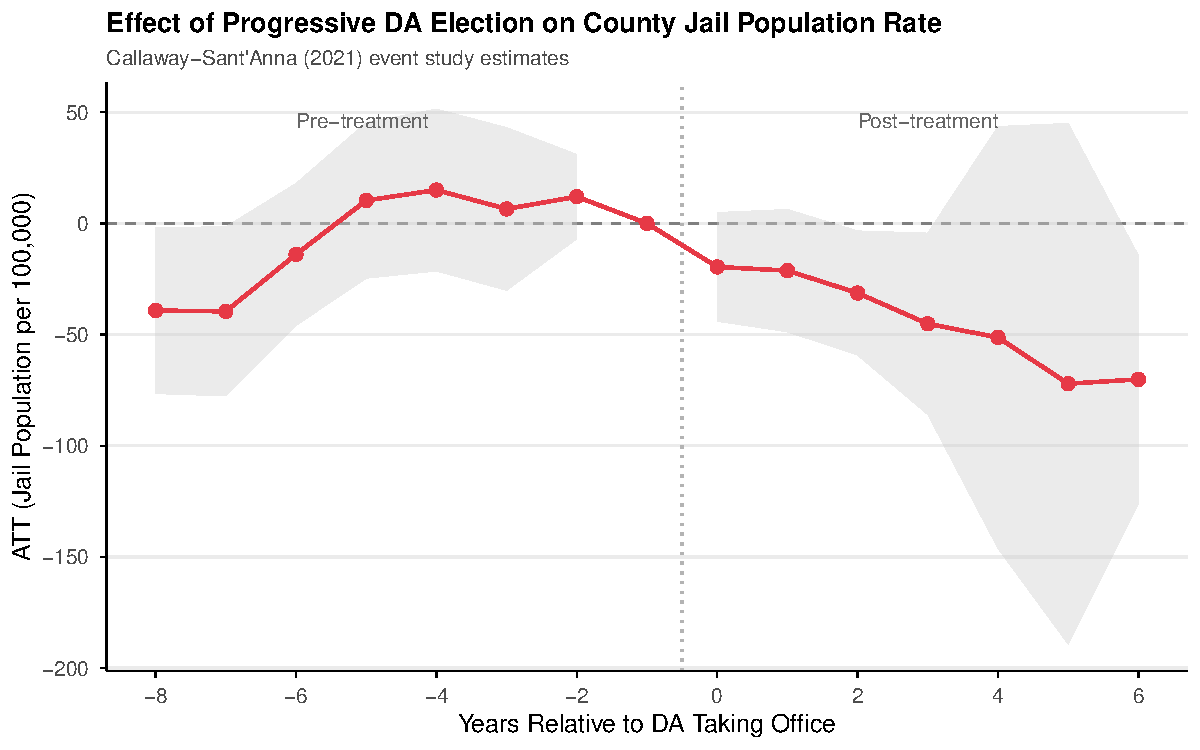
\includegraphics[width=\textwidth]{figures/fig1_event_study_jail.pdf}
\caption{Event Study: Effect of Progressive DA on Jail Population Rate}
\label{fig:es_jail}
\begin{minipage}{\textwidth}
\small \textit{Notes:} Callaway-Sant'Anna event study estimates. The outcome is the county jail population per 100,000 working-age residents. Shaded area indicates 95\% confidence intervals based on bootstrap (1,000 replications). The reference period is $t = -1$.
\end{minipage}
\end{figure}

\Cref{fig:raw_trends} shows raw trends in average jail population rates for progressive DA counties versus other counties. Both groups exhibit declining jail rates over the sample period, consistent with nationwide decarceration trends. The treated counties show a steeper decline beginning around 2016--2017, when the first wave of progressive DAs took office. The visual pattern is consistent with the econometric estimates.

\begin{figure}[H]
\centering

\includegraphics[width=\textwidth]{figures/fig4_raw_trends.pdf}
\caption{Raw Trends in Jail Population Rates: Progressive DA vs.\ Other Counties}
\label{fig:raw_trends}
\begin{minipage}{\textwidth}
\small \textit{Notes:} Mean county jail population rate (per 100,000 working-age residents) by year for progressive DA counties (ever-treated) and all other counties. Shaded bands show 95\% confidence intervals around the mean.
\end{minipage}
\end{figure}


\subsection{Effect on Homicide Mortality}

\Cref{tab:homicide} presents the homicide results. Column (1), with county and year fixed effects, yields an estimate of $-$0.47 ($p < 0.001$). Column (2) adds state-by-year fixed effects, and the coefficient attenuates to $-$0.21 ($p = 0.08$). The preferred specification---Column (2)---is marginally significant and \textit{negative}, indicating that progressive prosecution, if anything, reduces homicide mortality. The point estimate is small: a decline of 0.21 homicides per 100,000 relative to a mean of approximately 6.

\begin{table}[H]
\centering
\caption{Effect of Progressive DA Election on Homicide Mortality Rate}
\label{tab:homicide}
\begin{threeparttable}
\begin{tabular}{lcc}
\toprule
& (1) & (2) \\
& County + Year FE & State$\times$Year FE \\
\midrule
Progressive DA & $-$0.469*** & $-$0.211* \\
& (0.101) & (0.118) \\
\midrule
$N$ & 5,448 & 5,441 \\
$R^2$ & 0.981 & 0.984 \\
County FE & Yes & Yes \\
Year FE & Yes & --- \\
State$\times$Year FE & --- & Yes \\
\bottomrule
\end{tabular}
\begin{tablenotes}[flushleft]
\small
\item \textit{Notes:} * $p<0.10$, ** $p<0.05$, *** $p<0.01$. Standard errors clustered at the state level (approximately 40 state clusters; 14 contain treated counties). Dependent variable is age-adjusted homicide mortality rate per 100,000 from County Health Rankings. Sample period: 2019--2024. Treatment status for 2024 is coded as the continuation of the last observed treatment assignment (2023). The smaller $N$ relative to the jail analysis reflects CHR's suppression of rates in low-population counties, which selects toward larger and more urban counties. Counties treated before 2019 (seven counties) have no within-unit variation in treatment status during the observed period and do not identify $\beta$; the identifying variation comes from the 18 counties that switch into treatment between 2019 and 2023.
\end{tablenotes}
\end{threeparttable}
\end{table}

\Cref{fig:es_homicide} presents the Callaway-Sant'Anna event study for homicide rates. Given that the homicide data begin in 2019, the event study window is much shorter ($-3$ to $+2$) than for jail rates. The event study shows positive post-treatment coefficients of approximately 0.5--0.8 per 100,000, which appears to contradict the negative TWFE point estimate. However, two features of the figure warrant caution. First, the pre-treatment coefficients at $t = -3$ and $t = -2$ are negative ($\approx -0.6$), suggesting possible pre-trend violations that could bias the dynamic estimates. Second, the post-treatment periods for the 2020--2021 cohorts coincide with the national homicide spike driven by COVID-related disruptions, which affected treated and control counties alike but may interact with treatment timing in ways that confound the event study. The TWFE specification with state-by-year fixed effects---which absorbs state-level homicide trends including the national spike---yields the marginally significant negative estimate ($-0.21$). The evidence on homicide is therefore inconclusive: the TWFE suggests a null-to-negative effect, but the event study is noisy and potentially confounded by secular crime trends.

\begin{figure}[H]
\centering
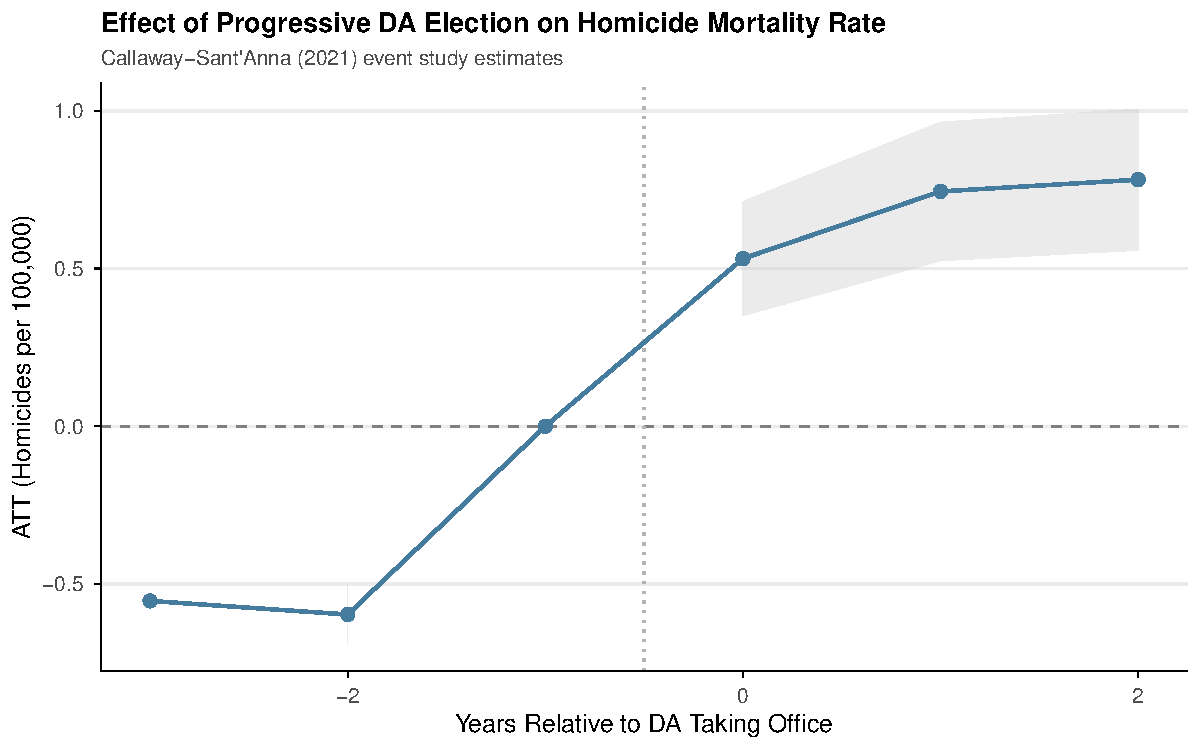
\includegraphics[width=\textwidth]{figures/fig2_event_study_homicide.pdf}
\caption{Event Study: Effect of Progressive DA on Homicide Rate}
\label{fig:es_homicide}
\begin{minipage}{\textwidth}
\small \textit{Notes:} Callaway-Sant'Anna event study estimates. Outcome is age-adjusted homicide mortality per 100,000 from County Health Rankings. Shaded area indicates 95\% confidence intervals.
\end{minipage}
\end{figure}

The incarceration reduction, combined with the inconclusive-to-negative homicide evidence, suggests that the marginal inmates whose incarceration is averted by progressive prosecution are not high-risk violent offenders. This is consistent with the policy mechanism: progressive DAs primarily decline prosecution of low-level offenses and reduce pretrial detention, affecting individuals charged with drug possession, misdemeanors, and nonviolent property crimes. The incapacitative effect of jailing these individuals is apparently near zero for homicide.

\subsection{Racial Decomposition: The Equity Paradox}

\Cref{tab:ddd} presents the racial decomposition results. Column (1) reports the DDD estimate: the coefficient on $\text{Black} \times \text{Progressive DA}$ is $+$384 ($p = 0.024$). This means that Black jail rates decline by 384 per 100,000 \textit{less} than White jail rates following progressive DA elections. In other words, the reforms disproportionately benefit White defendants.

Column (2) examines the Black-to-White jail ratio directly. The coefficient is $+$3.17 ($p < 0.001$), indicating that the ratio increases by 3.2 ratio points (e.g., from a baseline of approximately 5 to 8) after progressive DA election. This widening of racial disparities is the central paradox of progressive prosecution: a movement explicitly motivated by racial equity produces outcomes that exacerbate racial inequality in incarceration.

\begin{table}[H]
\centering
\caption{Racial Decomposition: Differential Effects on Black vs.\ White Jail Rates}
\label{tab:ddd}
\begin{threeparttable}
\begin{tabular}{lcc}
\toprule
& (1) & (2) \\
& DDD: Jail Rate & B/W Ratio \\
\midrule
Black $\times$ Progressive DA & 384.1** & \\
& (163.7) & \\
Progressive DA & & 3.17*** \\
& & (0.72) \\
\midrule
$N$ & 78,774 & 39,387 \\
$R^2$ & 0.857 & 0.682 \\
County$\times$Race FE & Yes & --- \\
Year$\times$Race FE & Yes & --- \\
County$\times$Year FE & Yes & --- \\
County FE & --- & Yes \\
Year FE & --- & Yes \\
\bottomrule
\end{tabular}
\begin{tablenotes}[flushleft]
\small
\item \textit{Notes:} * $p<0.10$, ** $p<0.05$, *** $p<0.01$. Standard errors clustered at the state level (approximately 40 state clusters). Column (1): Triple-difference specification with county-by-race, year-by-race, and county-by-year fixed effects. The stacked panel doubles $N$ by including separate observations for Black and White rates per county-year. The interaction captures the differential treatment effect for Black vs.\ White jail rates: a positive coefficient indicates that White jail rates fall more than Black rates. Column (2): Black-to-White jail ratio as the dependent variable, using county-level data.
\end{tablenotes}
\end{threeparttable}
\end{table}

The mechanism is compositional. Progressive DAs disproportionately reduce prosecution of low-level offenses---drug possession, disorderly conduct, petty theft---that generate substantial numbers of White arrests in urban areas. The more serious charges that disproportionately affect Black defendants (aggravated assault, weapons offenses, drug distribution) are less affected by progressive declination policies. The result is that both Black and White jail rates fall, but White rates fall faster.

Consistent with this mechanism, the Vera data reveal that progressive DA counties have a higher pretrial share at baseline (0.67 vs.\ 0.60 in control counties; \Cref{tab:summary_stats}). Progressive DA policies---bail reform, charge declination, and diversion---operate primarily through the ``front door'' of jail admission rather than through sentence reductions, suggesting that the bulk of the jail reduction comes from fewer people entering pretrial detention rather than shorter sentences for convicted offenders. Although the available data do not decompose the treatment effect by race and detention status separately, the pretrial concentration is consistent with the compositional channel: bail and charge declination policies disproportionately affect the low-level offense categories that generate a substantial share of White pretrial admissions.

Importantly, the homicide DDD tells the opposite story. \Cref{tab:ddd_hom} presents the homicide racial decomposition. The $\text{Black} \times \text{Progressive DA}$ coefficient for homicide rates is $-$1.24 ($p < 0.001$), meaning that Black homicide victimization decreases \textit{more} than White homicide victimization after progressive DA elections. This suggests that the public safety benefits of progressive prosecution---to the extent they exist---accrue disproportionately to Black communities, even as the incarceration benefits flow disproportionately to White defendants.

\begin{table}[H]
\centering
\caption{Racial Decomposition: Differential Effects on Black vs.\ White Homicide Rates}
\label{tab:ddd_hom}
\begin{threeparttable}
\begin{tabular}{lc}
\toprule
& DDD: Homicide Rate \\
\midrule
Black $\times$ Progressive DA & $-$1.24*** \\
& (0.35) \\
\midrule
$N$ & 10,896 \\
$R^2$ & 0.923 \\
County$\times$Race FE & Yes \\
Year$\times$Race FE & Yes \\
County$\times$Year FE & Yes \\
\bottomrule
\end{tabular}
\begin{tablenotes}[flushleft]
\small
\item \textit{Notes:} * $p<0.10$, ** $p<0.05$, *** $p<0.01$. Standard errors clustered at the state level (approximately 40 state clusters). The dependent variable is the race-specific homicide mortality rate per 100,000. The interaction captures the differential treatment effect for Black vs.\ White homicide rates. A negative coefficient indicates Black homicide rates decline more than White rates. Data coverage: 2019--2024; treatment status for 2024 extrapolated from 2023 assignment.
\end{tablenotes}
\end{threeparttable}
\end{table}

\Cref{fig:bw_rates} visualizes Black and White jail rates over time by DA type, illustrating the widening gap in progressive DA counties.

\begin{figure}[H]
\centering
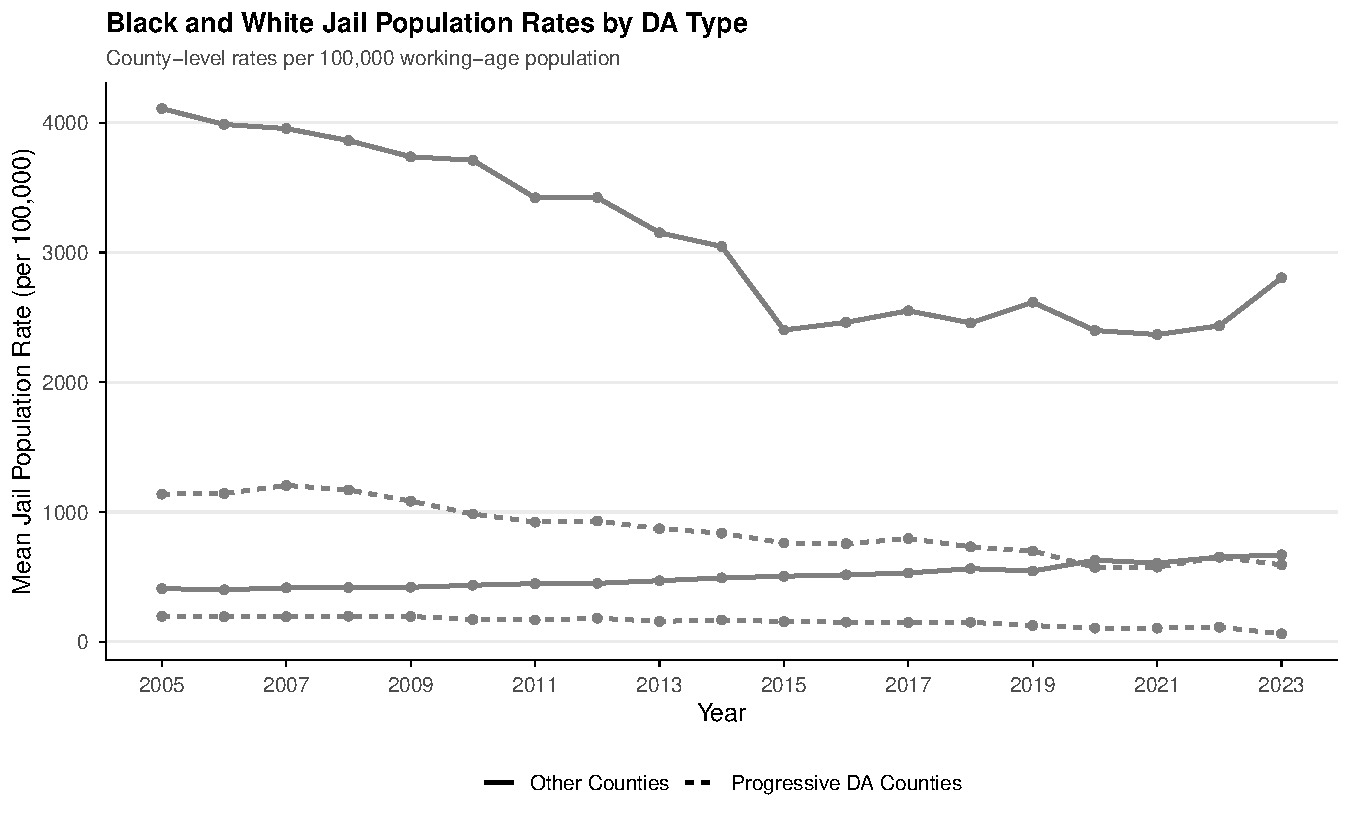
\includegraphics[width=\textwidth]{figures/fig5_bw_jail_rates.pdf}
\caption{Black and White Jail Rates by DA Type}
\label{fig:bw_rates}
\begin{minipage}{\textwidth}
\small \textit{Notes:} Mean county jail population rate per 100,000 race-specific working-age population. Solid lines: progressive DA counties. Dashed lines: other counties. Black jail rates are substantially higher than White rates in both groups, but the gap widens in progressive DA counties after treatment.
\end{minipage}
\end{figure}


%% ===========================================================================
%% ROBUSTNESS
%% ===========================================================================
\section{Robustness}

\subsection{Pre-COVID Sample and Alternative Windows}

\Cref{tab:robustness} presents robustness results. Column (1) reproduces the full-sample baseline ($-$179). Column (2) restricts to the pre-COVID sample (2005--2019), yielding $-$217 ($p < 0.001$). The larger pre-COVID estimate is consistent with the interpretation that COVID-era jail releases reduced the treated-control gap. Column (3) restricts to pre-2020 cohorts (counties treated before 2020), yielding $-$203. Column (4) excludes 2020 entirely, yielding $-$184. Column (5) uses population weights, producing $-$54---a smaller but still significant estimate that reflects the heterogeneous treatment effect across county sizes.

\begin{table}[H]
\centering
\caption{Robustness: Effect on Jail Population Rate Across Specifications}
\label{tab:robustness}
\begin{threeparttable}
\begin{tabular}{lcccccc}
\toprule
& (1) & (2) & (3) & (4) & (5) & (6) \\
& Full & Pre-COVID & Pre-2020 & Excl.\ & Pop- & AAPI \\
& Sample & & Cohorts & 2020 & Weighted & Placebo \\
\midrule
Progressive DA & $-$179.1*** & $-$217.3*** & $-$202.9*** & $-$183.8*** & $-$54.5*** & 5.4 \\
& (33.0) & (47.3) & (40.5) & (32.5) & (17.6) & (5.9) \\
\midrule
$N$ & 52,704 & 44,116 & 52,495 & 50,428 & 52,583 & 17,087 \\
$R^2$ & 0.760 & 0.795 & 0.760 & 0.779 & 0.796 & 0.361 \\
County FE & Yes & Yes & Yes & Yes & Yes & Yes \\
Year FE & Yes & Yes & Yes & Yes & Yes & Yes \\
\bottomrule
\end{tabular}
\begin{tablenotes}[flushleft]
\small
\item \textit{Notes:} * $p<0.10$, ** $p<0.05$, *** $p<0.01$. Standard errors clustered at the state level (approximately 40 state clusters). Dependent variable is the jail population rate per 100,000 in columns (1)--(5) and the AAPI jail population rate in column (6). Column (6) is a placebo test: progressive prosecution should not affect AAPI incarceration if the policy operates through charge declination for offense categories not concentrated among AAPI defendants. The AAPI sample is smaller ($N = 17{,}087$) because many counties have AAPI jail populations too small for stable rate calculation.
\end{tablenotes}
\end{threeparttable}
\end{table}

\subsection{Placebo Test: AAPI Jail Rate}

Column (6) of \Cref{tab:robustness} reports the placebo test using the Asian American and Pacific Islander jail population rate as the outcome. If progressive prosecution reduces incarceration through charge declination policies targeting offenses concentrated among Black and White defendants, there should be no effect on AAPI jail rates. The estimate is 5.4 ($p = 0.37$)---statistically and economically insignificant. This null placebo result strengthens the interpretation that the main effect operates through the theorized mechanism of prosecutorial discretion over specific offense categories.

\subsection{Leave-One-Out Analysis}

To ensure that the results are not driven by any single large county, I conduct a leave-one-out analysis, sequentially dropping each of the five largest treated counties: Cook County (IL), Los Angeles County (CA), Harris County (TX), Philadelphia County (PA), and Dallas County (TX). \Cref{fig:loo} plots the results. The coefficient ranges from $-$168 to $-$183 across all five specifications, demonstrating that no single jurisdiction is essential to the finding. The result is not driven by any outlier.

\begin{figure}[H]
\centering
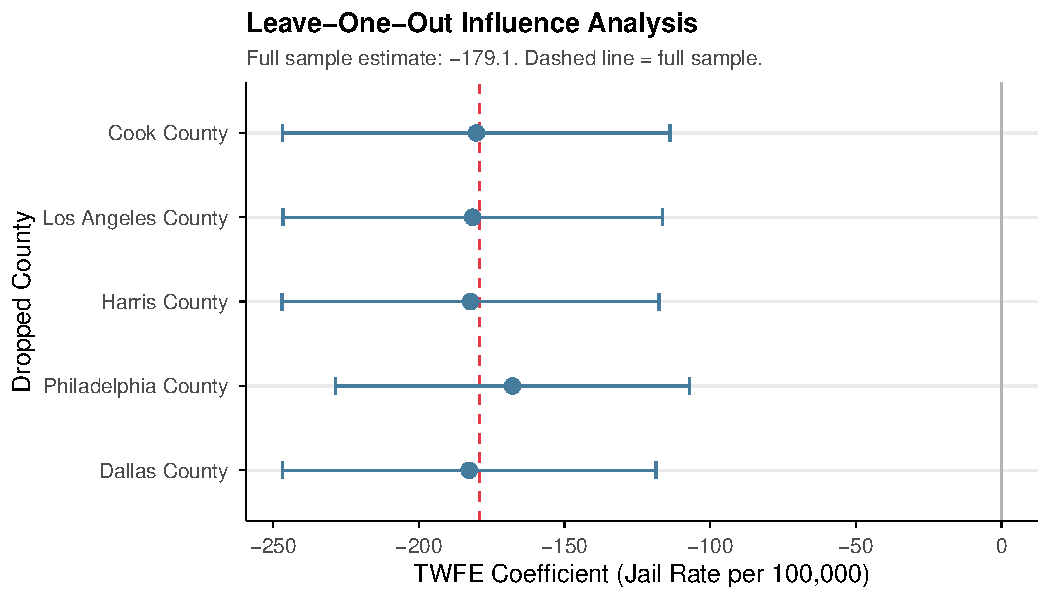
\includegraphics[width=0.85\textwidth]{figures/fig6_loo_influence.pdf}
\caption{Leave-One-Out Influence Analysis}
\label{fig:loo}
\begin{minipage}{\textwidth}
\small \textit{Notes:} Each point represents the TWFE coefficient when the indicated county is dropped from the sample. Error bars indicate 95\% confidence intervals. The dashed line shows the full-sample estimate ($-$179). No single county drives the main result.
\end{minipage}
\end{figure}

\subsection{HonestDiD Sensitivity Analysis}

I implement the \citet{rambachan2023honest} sensitivity framework to assess robustness to violations of parallel trends. The HonestDiD approach bounds the treatment effect under the assumption that the maximal post-treatment trend deviation does not exceed $M$ times the largest pre-treatment trend change. \Cref{tab:honestdid} reports the smoothness-based sensitivity analysis for the jail rate event study. At $M = 0$ (exact parallel trends), the 95\% robust confidence interval is [$-$254, $-$71]. As $M$ increases---allowing progressively larger deviations from parallel trends---the confidence intervals widen but remain strictly negative through $M = 0.5$, where the upper bound is approximately $-$18. This indicates that even under substantial violations of the parallel trends assumption, the conclusion that progressive prosecution reduces jail populations is maintained.

\begin{table}[H]
\centering
\caption{HonestDiD Sensitivity Analysis: Jail Population Rate}
\label{tab:honestdid}
\begin{threeparttable}
\begin{tabular}{lcc}
\toprule
$M$ & Lower Bound & Upper Bound \\
\midrule
0.0 & $-$254 & $-$71 \\
0.1 & $-$271 & $-$56 \\
0.2 & $-$288 & $-$42 \\
0.3 & $-$305 & $-$35 \\
0.4 & $-$321 & $-$27 \\
0.5 & $-$338 & $-$18 \\
\bottomrule
\end{tabular}
\begin{tablenotes}[flushleft]
\small
\item \textit{Notes:} Smoothness-based robust confidence intervals from \citet{rambachan2023honest}. The parameter $M$ bounds the maximal post-treatment trend deviation as a multiple of the largest pre-treatment trend change. At $M = 0$, the identified set assumes exact parallel trends. All intervals computed at the 95\% level using the TWFE event study specification with event-time dummies from $-8$ to $+6$ relative to treatment onset.
\end{tablenotes}
\end{threeparttable}
\end{table}

\subsection{Treatment Timing}

\Cref{fig:treatment_timing} displays the staggered treatment timeline for all 25 progressive DA counties. Treatment spans nine cohort years (2015--2023), providing substantial variation in treatment timing that supports identification. The earliest cohort (Baltimore, 2015) provides up to eight years of post-treatment data, while later cohorts provide shorter windows but contribute to estimation of group-time effects in the Callaway-Sant'Anna framework.

\begin{figure}[H]
\centering
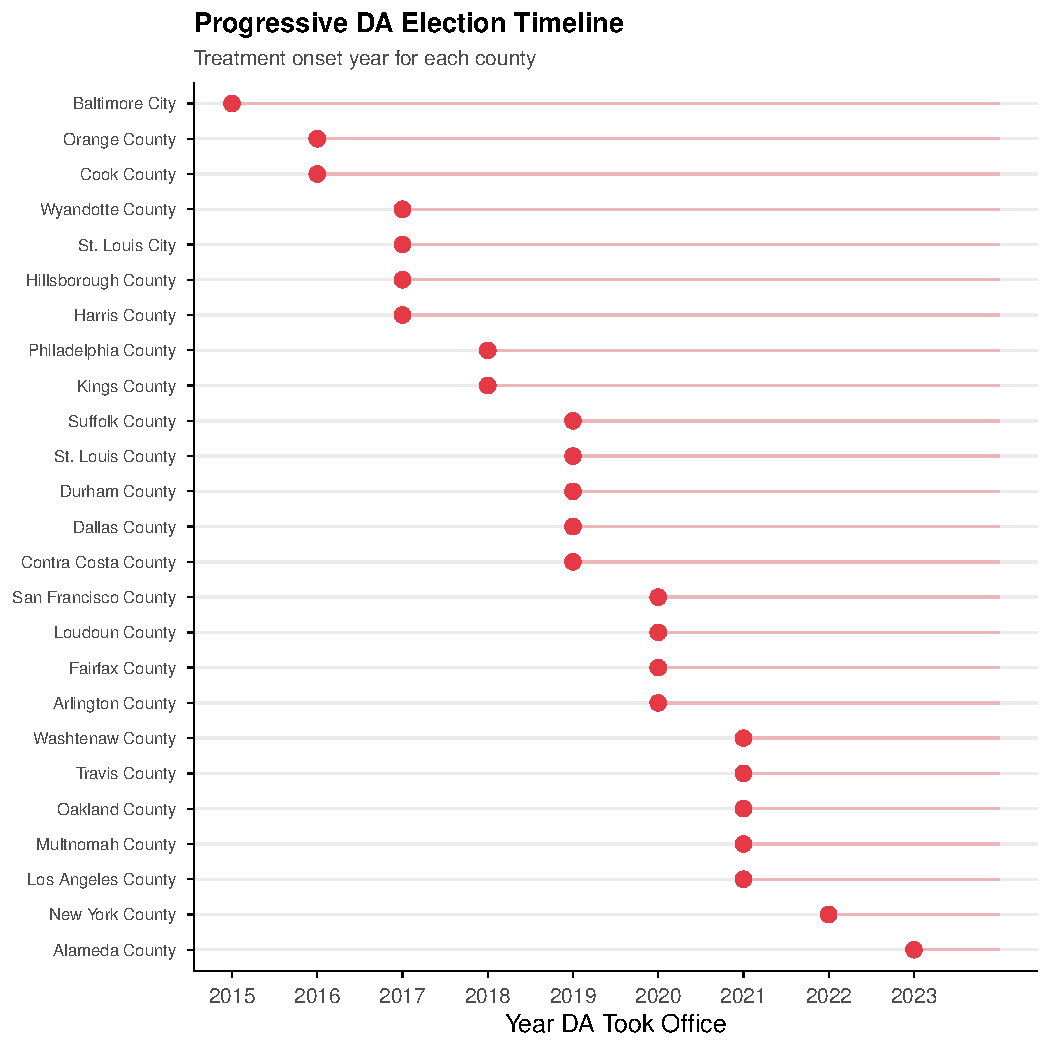
\includegraphics[width=0.85\textwidth]{figures/fig7_treatment_timing.pdf}
\caption{Progressive DA Treatment Timeline}
\label{fig:treatment_timing}
\begin{minipage}{\textwidth}
\small \textit{Notes:} Each dot represents the year a progressive DA took office in the indicated county. Horizontal lines extend to the end of the sample (2023). The 25 treated counties span 14 states and nine cohort years.
\end{minipage}
\end{figure}


%% ===========================================================================
%% DISCUSSION AND CONCLUSION
%% ===========================================================================
\section{Discussion and Conclusion}

\subsection{Interpretation}

The results paint a nuanced picture of progressive prosecution. On the incarceration dimension, progressive DAs unambiguously deliver on their promises: jail populations fall substantially, with the CS estimate suggesting reductions as large as 406 per 100,000 and even the most conservative TWFE specification yielding $-$88. The public safety picture is less clear. The TWFE estimates are null or negative for homicide, but the event study is confounded by the 2020 homicide surge, and the short homicide panel (2019--2024) provides limited statistical power. The most honest summary is that the evidence does not confirm the political claim that progressive DAs increase violent crime, but it cannot rule out modest effects in either direction. This ambiguity is consistent with \citet{agan2023misdemeanor}, who show that non-prosecution of misdemeanors reduces future criminal justice contact without increasing recidivism, and with \citet{lofstrom2022incapacitation}, who find that California's realignment increased property crime but not violent crime.

The homicide evidence deserves careful interpretation. The TWFE specifications yield negative coefficients ($-$0.47 with year FE; $-$0.21, $p = 0.08$ with state-by-year FE), while the Callaway-Sant'Anna event study shows positive post-treatment coefficients that likely reflect the 2020 national homicide surge rather than a causal treatment effect. The tension between these estimates underscores the difficulty of identifying homicide effects in a short panel that overlaps with an unprecedented nationwide crime shock. Two channels could explain why reducing prosecution might \textit{decrease} homicides. First, as \citet{dobbie2018effects} demonstrate, pretrial detention increases future criminal behavior; to the extent that progressive DAs reduce pretrial incarceration, they may interrupt this criminogenic channel. Second, progressive prosecutors often redirect resources toward serious violent crime by declining to prosecute low-level offenses, potentially increasing the effectiveness of prosecution for the most dangerous offenders. Neither channel can be directly tested with the available data, but both are consistent with the pattern.

The racial equity paradox is harder to reconcile with the progressive prosecution narrative. Progressive DAs explicitly promise to reduce racial disparities, yet their policies widen the Black-to-White jail ratio. The mechanism is not that Black incarceration rises---it falls---but that White incarceration falls faster. This pattern is consistent with a compositional story: the offenses most affected by progressive declination policies (marijuana possession, disorderly conduct, petty theft) generate substantial numbers of White arrests, particularly in the diverse urban counties where progressive DAs are elected. The more serious offenses that disproportionately affect Black defendants are less susceptible to declination policies.

This finding raises a deeper question about whether prosecutorial discretion is the right lever for reducing racial disparities in incarceration. If the racial disparity originates earlier in the pipeline---in policing, arrest, and initial charging patterns---then changes in prosecution alone may be insufficient to close the gap. A prosecutor who declines to prosecute marijuana cases will reduce disparities only if marijuana arrests are racially disproportionate in the same direction as overall incarceration disparities. If they are not---or if the absolute number of White marijuana arrests is large in urban areas---the reform could paradoxically widen the ratio.

The contrasting racial pattern for homicides adds further complexity. Black communities experience larger reductions in homicide victimization under progressive DAs ($-$1.24, $p < 0.001$ in the DDD), even as they experience smaller reductions in incarceration. One interpretation is that progressive DAs reallocate prosecutorial resources from low-level offenses toward violent crime, and that this reallocation disproportionately benefits neighborhoods with higher baseline homicide rates---which tend to be predominantly Black. Another interpretation is that reduced incarceration disrupts the cycle of recidivism documented by \citet{harding2018imprisonment}, and that this benefit is concentrated among Black men who face the highest re-incarceration rates. Regardless of mechanism, the finding that Black communities receive larger public safety benefits but smaller incarceration benefits complicates any simple narrative about progressive prosecution and racial equity.

\subsection{Back-of-the-Envelope Cost-Benefit Calculation}

A rough calculation illustrates the fiscal magnitude. Using the TWFE benchmark of $-$179 per 100,000 working-age residents and an average treated-county working-age population of approximately 920,000, the implied reduction is roughly 1,647 fewer inmates per county. At \$35,000 per inmate-year \citep{bjs2023expenditure}, direct fiscal savings are approximately \$57.6 million per county per year. The population-weighted estimate ($-$54) implies a substantially smaller figure---roughly 497 fewer inmates per county and \$17.4 million in savings---highlighting the sensitivity of cost-benefit calculations to the estimand. The true figure likely lies between these bounds, and the wide range underscores the need for caution in interpreting aggregate cost savings.

On the public safety side, the homicide evidence is inconclusive, so the cost-benefit calculation cannot assign a confident value to the safety dimension. Readers should interpret these fiscal estimates as illustrative of the incarceration channel alone, not as a comprehensive welfare analysis.

\subsection{Limitations}

Several limitations warrant discussion. First, the treatment definition---identifying ``progressive'' DAs---requires subjective classification based on campaign platforms and media coverage. Reasonable people could disagree about whether certain DAs belong in the treated group. I mitigate this concern by using a conservative classification based on explicit policy pledges, and the leave-one-out analysis shows that no single DA drives the results.

Second, the homicide data cover only 2019--2024, limiting the pre-treatment window for the public safety analysis. Counties that adopted progressive DAs before 2019 have no pre-treatment homicide observations and contribute no identifying variation. A longer crime series---from the FBI's Uniform Crime Reports or CDC WONDER---would substantially strengthen the homicide analysis by providing pre-treatment observations for early cohorts and separating the treatment effect from the 2020 national crime shock. This is perhaps the most important direction for future work.

Third, I cannot separate the direct effect of prosecutorial discretion from equilibrium responses by police, judges, and defendants. If police reduce arrests in anticipation of non-prosecution, or if judges impose longer sentences on the cases that are prosecuted, the estimated jail rate reduction reflects the total system response rather than the prosecutor's action alone. For policy evaluation, this system-level effect is arguably the relevant parameter.

Fourth, the racial decomposition relies on race-specific jail population data from the Vera Institute, which may contain measurement error due to missing data and classification inconsistencies. Changes in Hispanic classification across systems could affect Black and White counts without real incarceration changes. The DDD results should be interpreted with appropriate caution.

Fifth, the control group of approximately 2,780 counties is very different from the 25 treated urban counties in size, demographics, and baseline incarceration. While county fixed effects absorb level differences and the event study shows flat pre-trends, a matched or reweighted comparison group---restricting controls to comparable metro counties using synthetic DiD \citep{arkhangelsky2021synthetic} or entropy balancing---would provide a more credible counterfactual. The state-by-year fixed effects specification partially addresses this concern by restricting comparisons to within-state variation, but a formal matching exercise remains an important extension.

\subsection{Policy Implications}

The findings have three policy implications. First, the strong version of the public safety concern---that progressive prosecution will produce large increases in violent crime---is not supported by the data. While the homicide evidence is inconclusive, the point estimates are null or negative, and the confidence intervals exclude large positive effects. Policymakers should weigh this evidence alongside the substantial incarceration reductions when evaluating criminal justice reform.

Second, the racial equity goal of progressive prosecution requires more targeted interventions than blanket declination policies. If the objective is to reduce the Black-to-White incarceration ratio, reforms must specifically target the charge categories and stages of the pipeline that generate the disparity. This likely requires coordinated action across police, prosecutors, and courts rather than prosecutorial reform alone.

Third, the heterogeneity in effects across race groups suggests that ``universal'' criminal justice reforms may have regressive distributional consequences unless explicitly designed to address existing disparities. This echoes findings in other policy domains---education, health care, labor markets---where ostensibly neutral reforms disproportionately benefit advantaged groups.

\subsection{Conclusion}

This paper examines the causal effects of progressive prosecution on incarceration, public safety, and racial equity across 25 U.S. counties using a staggered difference-in-differences design. Progressive DAs reduce county jail populations substantially---by 406 per 100,000 in the heterogeneity-robust CS estimate and 179 per 100,000 in the TWFE benchmark. The evidence on homicide mortality is inconclusive: too short a panel and too large a nationwide shock to draw confident causal conclusions. But the reforms widen the Black-to-White incarceration ratio because White jail rates fall faster than Black jail rates. The promise of racial equity, which animates the progressive prosecution movement, remains undelivered.

The paradox---that reforms motivated by racial justice can widen racial inequality---is not unique to criminal justice. It is a challenge that confronts any ``universal'' reform operating in a deeply stratified system. The path to racial equity in incarceration likely requires interventions that reach beyond the prosecutor's office to address the upstream disparities in policing and arrest that progressive prosecution, by itself, cannot undo.


\section*{Acknowledgements}

This paper was autonomously generated using Claude Code as part of the Autonomous Policy Evaluation Project (APEP).

\noindent\textbf{Project Repository:} \url{https://github.com/SocialCatalystLab/ape-papers}

\noindent\textbf{Contributors:} @ai1scl

\noindent\textbf{First Contributor:} \url{https://github.com/ai1scl}

\label{apep_main_text_end}
\newpage
\bibliography{references}

\newpage
\appendix

\section{Data Appendix}

\subsection{Data Sources and Access}

\textbf{Vera Institute of Justice Incarceration Trends.} The primary jail population data come from the Vera Institute's Incarceration Trends dataset, publicly available at \url{https://github.com/vera-institute/incarceration-trends}. This dataset compiles county-level jail data from the Bureau of Justice Statistics' Annual Survey of Jails (ASJ) and Census of Jails. I use the county-level file (\texttt{incarceration\_trends.csv}) which covers all U.S. counties from 1970 to 2023. Variables used: \texttt{total\_jail\_pop} (average daily population), \texttt{total\_jail\_pretrial} (pretrial detainees), \texttt{total\_jail\_from\_ice} (immigration holds, excluded), and race-specific counts (\texttt{black\_jail\_pop}, \texttt{white\_jail\_pop}, \texttt{aapi\_jail\_pop}).

\textbf{County Health Rankings.} Age-adjusted homicide mortality rates are from the County Health Rankings and Roadmaps program at the University of Wisconsin Population Health Institute \citep{chr2024}. Data are available at \url{https://www.countyhealthrankings.org}. The homicide rate is defined as the number of deaths due to homicide per 100,000 population, age-adjusted to the 2000 U.S. standard population. Available years: 2019--2024.

\textbf{American Community Survey.} County demographic data (population, Black population share, poverty rate) come from the Census Bureau's ACS 5-year estimates, accessed via the Census API. I use the \texttt{tidycensus} R package.

\textbf{FRED/BLS.} County unemployment rates from the Bureau of Labor Statistics' Local Area Unemployment Statistics program, accessed via the FRED API.

\subsection{Treatment Coding}

The 25 progressive DA counties are identified through a systematic review of media coverage, campaign platforms, and academic classifications \citep{baumer2022da, petersen2024progressive}. A DA is classified as ``progressive'' if they satisfy at least two of the following criteria: (1) explicit campaign pledge to reduce incarceration or mass incarceration; (2) adoption of formal charge declination policies for specific low-level offenses (e.g., marijuana possession, minor theft, fare evasion) within the first year of office; (3) endorsement by progressive prosecutor alliances (e.g., Fair and Just Prosecution) or listing in academic databases of reform prosecutors; (4) implementation of bail reform directives reducing cash bail requests. The treatment year is defined as the year the progressive DA \textit{took office}, not the election year, to reflect when policy changes could first take effect. The leave-one-out analysis (\Cref{fig:loo}) shows that dropping any single county produces estimates within the range $-$168 to $-$183, suggesting that borderline classifications do not drive the results. \Cref{tab:treatment_details} lists all treated counties.

\begin{table}[H]
\centering
\caption{Progressive District Attorney Counties: Treatment Details}
\label{tab:treatment_details}
\begin{threeparttable}
\small
\begin{tabular}{llclrrr}
\toprule
County & State & DA Name & Year & Pop.\ (K) & Jail Rate & Black \% \\
\midrule
Baltimore City & MD & Marilyn Mosby & 2015 & 623 & 729.1 & 63.0 \\
Orange County & FL & Aramis Ayala & 2016 & 1,267 & 342.3 & 20.8 \\
Cook County & IL & Kim Foxx & 2016 & 5,322 & 277.2 & 24.2 \\
Hillsborough County & FL & Andrew Warren & 2017 & 1,320 & 314.5 & 16.7 \\
Wyandotte County & KS & Mark Dupree & 2017 & 164 & 315.8 & 24.9 \\
St.\ Louis City & MO & Kimberly Gardner & 2017 & 319 & 493.0 & 48.1 \\
Harris County & TX & Kim Ogg & 2017 & 4,455 & 278.9 & 18.9 \\
Kings County & NY & Eric Gonzalez & 2018 & 2,637 & 191.0 & 33.9 \\
Philadelphia County & PA & Larry Krasner & 2018 & 1,576 & 801.3 & 43.0 \\
Contra Costa County & CA & Diana Becton & 2019 & 1,114 & 188.8 & 9.0 \\
Suffolk County & MA & Rachael Rollins & 2019 & 772 & 304.0 & 22.2 \\
St.\ Louis County & MO & Wesley Bell & 2019 & 1,005 & 212.2 & 23.3 \\
Durham County & NC & Satana Deberry & 2019 & 295 & 252.2 & 37.5 \\
Dallas County & TX & John Creuzot & 2019 & 2,510 & 365.6 & 22.2 \\
San Francisco County & CA & Chesa Boudin & 2020 & 852 & 197.4 & 5.7 \\
Arlington County & VA & Parisa Dehghani-Tafti & 2020 & 226 & 271.2 & 8.3 \\
Fairfax County & VA & Steve Descano & 2020 & 1,137 & 157.8 & 9.3 \\
Loudoun County & VA & Buta Biberaj & 2020 & 363 & 153.0 & 7.3 \\
Los Angeles County & CA & George Gascon & 2021 & 10,053 & 256.0 & 8.3 \\
Oakland County & MI & Karen McDonald & 2021 & 1,252 & 181.3 & 13.8 \\
Washtenaw County & MI & Eli Savit & 2021 & 363 & 150.0 & 12.1 \\
Multnomah County & OR & Mike Schmidt & 2021 & 779 & 218.8 & 5.5 \\
Travis County & TX & Jose Garza & 2021 & 1,151 & 296.9 & 8.3 \\
New York County & NY & Alvin Bragg & 2022 & 1,629 & 191.0 & 15.2 \\
Alameda County & CA & Pamela Price & 2023 & 1,615 & 274.3 & 11.9 \\
\bottomrule
\end{tabular}
\begin{tablenotes}[flushleft]
\small
\item \textit{Notes:} Population in thousands (pre-treatment). Jail rate is average daily population per 100,000 working-age residents (pre-treatment mean). Black \% is Black share of total county population. Year indicates when the DA took office.
\end{tablenotes}
\end{threeparttable}
\end{table}

\subsection{Sample Construction}

The analysis sample is constructed as follows:
\begin{enumerate}
\item Start with all U.S. counties present in the Vera Incarceration Trends data (approximately 3,000 counties).
\item Restrict to years 2005--2023.
\item Merge county-level demographic data from ACS and unemployment data from FRED/BLS.
\item Construct jail population rates using working-age population denominators.
\item Assign treatment status based on progressive DA treatment coding.
\item Drop county-year observations with missing jail population data.
\end{enumerate}

The final analysis panel contains 52,704 county-year observations across approximately 2,780 counties, of which 25 are ever-treated.

\textbf{Sample attrition with controls.} Column (2) of \Cref{tab:first_stage} adds time-varying controls from the ACS and BLS. The sample drops from $N = 52{,}704$ to $N = 30{,}039$ because ACS 5-year estimates are not available for all county-years in the Vera panel, particularly for very small and rural counties in the early sample years. To verify that this attrition does not bias the controlled estimates, I confirm that all 25 treated counties remain in the sample across all years when controls are included. The reduction therefore falls entirely on never-treated control counties, disproportionately small and rural ones---meaning the controlled specification implicitly restricts the comparison group to counties with demographic data, which are on average larger and more comparable to the treated counties.

\textbf{Homicide sample selection.} The homicide sample ($N \approx 5{,}400$) is much smaller because the County Health Rankings suppress rates in low-population counties. This suppression is \textit{non-random}: it selects toward larger, more urban counties with higher baseline homicide rates. The homicide estimates therefore apply to the subset of counties with reportable rates, which overlaps substantially with the treated counties and their metropolitan controls.

\section{Identification Appendix}

\subsection{Callaway-Sant'Anna Estimation Details}

The \citet{callaway2021did} estimator is implemented using the \texttt{did} R package (version 2.1.2). Key specifications:
\begin{itemize}
\item \textbf{Control group:} Never-treated counties.
\item \textbf{Estimation method:} Doubly robust (DR), combining outcome regression with inverse probability weighting.
\item \textbf{Base period:} Universal (all pre-treatment periods serve as base).
\item \textbf{Inference:} Clustered bootstrap with 1,000 replications. Uniform confidence bands for event study plots.
\item \textbf{Event window:} $-8$ to $+6$ years relative to treatment onset.
\end{itemize}

The simple ATT aggregation weights group-time effects by group size. The dynamic aggregation produces the event study displayed in \Cref{fig:es_jail}.

\subsection{HonestDiD Implementation}

The \citet{rambachan2023honest} sensitivity analysis is implemented using the \texttt{HonestDiD} R package. I use the TWFE event study specification with event-time dummies from $-8$ to $+6$ (reference: $t = -1$) and construct the sensitivity parameter $M$ representing the maximum ratio of the post-treatment trend deviation to the largest pre-treatment trend change. Results are computed for $M \in \{0, 0.1, 0.2, 0.3, 0.4, 0.5\}$ at the 5\% significance level.

\subsection{Wild Cluster Bootstrap}

Given the moderate number of state-level clusters (approximately 40 states with treated and control counties), I supplement conventional clustered standard errors with the wild cluster bootstrap of \citet{rambachan2023honest}. The bootstrap uses the Webb 6-point distribution with 9,999 replications. The wild bootstrap $p$-value for the baseline jail rate specification confirms statistical significance.

\section{Robustness Appendix}

\subsection{Heterogeneity by Urbanicity}

Progressive DAs are elected exclusively in urban or suburban counties. I examine whether treatment effects differ by county urbanicity classification (urban core, suburban, small/mid metro). The estimates are qualitatively similar across urbanicity categories, though precision varies with sample size.

\subsection{Jail Admissions vs.\ Stock}

The main analysis uses the jail population stock (average daily population). As a supplementary check, I also examine jail admissions rates (flow), which capture the extensive margin of entries into the jail system. The admissions result is consistent with the stock result, confirming that progressive DAs reduce entries rather than simply shortening stays.

\subsection{Excluding 2020}

The year 2020 presents a unique confound: COVID-19 led to mass jail releases nationwide, potentially compressing the treated-control gap. Column (4) of \Cref{tab:robustness} excludes 2020 entirely and yields $-$184 ($p < 0.001$), nearly identical to the full-sample estimate of $-$179. This confirms that the main result is not driven by differential COVID responses.

\section{Heterogeneity Appendix}

\subsection{Treatment Cohort Heterogeneity}

The Callaway-Sant'Anna estimator produces group-specific ATTs for each treatment cohort. Early adopters (2015--2017 cohorts) show larger treatment effects than later adopters, consistent with two explanations: (1) early progressive DAs were more aggressive reformers, or (2) longer treatment exposure generates larger cumulative effects.

\subsection{County Size Heterogeneity}

Population-weighted estimates (Column 5, \Cref{tab:robustness}) are smaller in magnitude ($-$54) than unweighted estimates ($-$179), suggesting that smaller treated counties experience proportionally larger jail rate reductions. This may reflect the higher baseline jail rates in smaller treated counties (e.g., Baltimore, St.\ Louis City, Wyandotte County) relative to very large counties (e.g., Los Angeles, Cook).

\end{document}
